\section{Auswertung}
\label{sec:Auswertung}
In \autoref{fig:kennlinie1} und \autoref{fig:kennlinie2} sind die fünf gemessenen Kennlinien der Hochvakuumdiode
aufgetragen. Aus Gründen der Lesbarkeit wurden die Kennlinien auf zwei Plots aufgeteilt. Die dazu entsprechenden
Messwerte sind im Anhang zu finden. Der Sättigungswert wird als Maximum der Kennlinie bestimmt. Insgesamt fällt
auf, dass alle bis auf die Kennlinie für die maximale Heizstromstärke $I_{\symup{H}}=\SI{2,5}{\ampere}$ den zu
erwartenen Verlauf aufweisen. Daraus lässt sich folgern, dass der Sättigungswert hier nur als grobe Näherung
betrachtet werden kann.
\begin{figure}
  \centering
  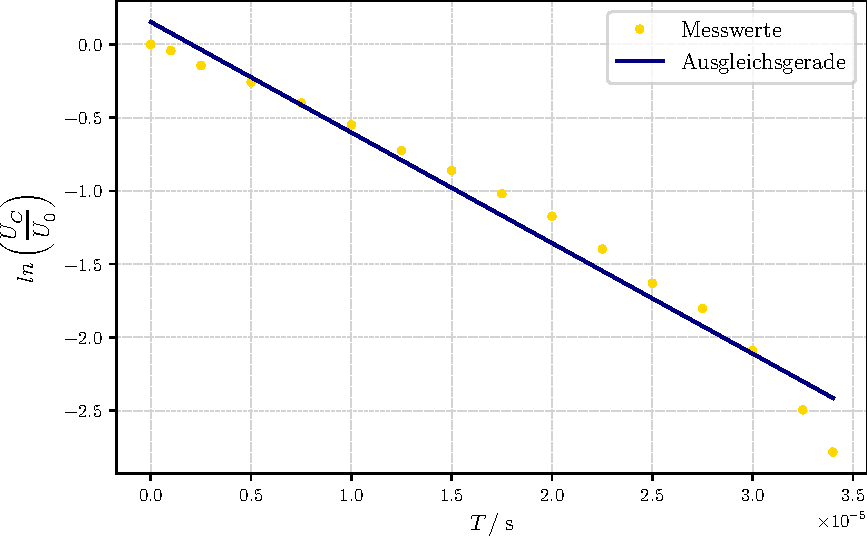
\includegraphics{plot1.pdf}
  \caption{Zwei Kennlinien der Hochvakuumdiode.}
  \label{fig:kennlinie1}
\end{figure}

\begin{figure}
  \centering
  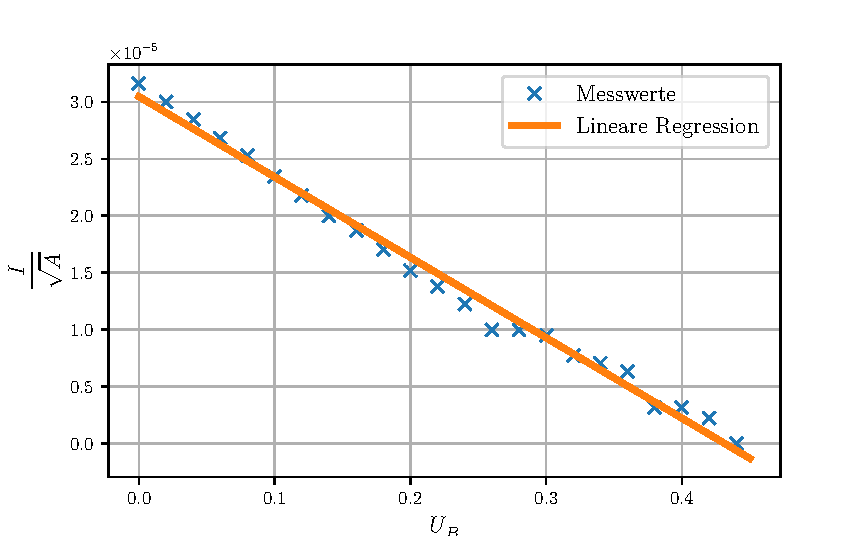
\includegraphics{plot2.pdf}
  \caption{Drei Kennlinien der Hochvakuumdiode.}
  \label{fig:kennlinie2}
\end{figure}
Die Sättigungswerte sind in \autoref{tab:saettigungswerte} dargestellt.
\begin{table}
  \centering
  \caption{Sättigungswerte der Kennlinien}
  \label{tab:saettigungswerte}
  \begin{tabular}{c c}
    \toprule
    $I_{\symup{H}}/\si{\ampere}$ & $I_{\symup{S}}/\si{\milli\ampere}$ \\
    \midrule
    1,9 & 0,052 \\
    2,0 & 0,199 \\
    2,1 & 0,294 \\
    2,3 & 1,289 \\
    2,5 & 3,020 \\
    \bottomrule
  \end{tabular}
\end{table}

\subsection{Gültigkeit des Langmuir-Schottkyschen Raumladungsgesetzes}
\label{sec:Langmuir}